\documentclass[12pt]{report}
\usepackage{url}
\usepackage{hyperref}
\usepackage{graphicx}
\usepackage{comment}
\usepackage{enumerate}
\usepackage[top=1.0in, bottom=1.0in, left=1.5in, right=1.5in]{geometry}
\title{Online Help Solution for The War Z}
\author{Sean McLellan\\ SE4HC3\\ McMaster University}
\date{\today}
\parskip=8pt
\begin{document}
\maketitle

\chapter{Introduction}

\section{Description of Software}
The online help solution is being developed for a Windows OS program called The War Z. This is a video game where the objective for the player is to survive the elements of the world, fighting off hordes of zombies and other human players while also preserving your own energy through the means of managing health, hunger, and thirst. The reason that an online help solution is suitable for this program specifically relates to the fact that there are no training modules for completely new players. They are simply placed in the world and left to fend for themselves, without a proper training module the difficulty curve may be too high for many new players to even try the game. Many things in the game are not as intuitive as one may think, and much of the game is left to trial-and-error, however with a proper online help solution players should be able to understand the mechanics of the game better and know what to do while in game rather than walk around aimlessly.

\chapter{Overview of Interface}
\section{Building Tool}
The building tool used to develop the online help solution is called Adobe Flash Creative Suite 3. This tool was chosen for a few reasons, one of which was because it is easy to develop with and is very modular due to the ability to add and remove \textit{scenes} and \textit{frames}. Scenes are parts of the project that may contain unrelated content or display information in a different format compared to another scene (i.e. the main menu of a game compared to the actual game mode itself). Frames are portions of a scene that can contain different but related content to the rest of the scene. With the combination of these two elements its very easy to design a hierarchical structure for a tutorial module using steps. It is also very easy to incorporate navigation tools into the module using the idea of frames and scenes. The ability to place and arrange pieces of the UI for the tutorial module is also very simple to do in Flash because there are no constraints on formatting, the only thing for a designer to be aware of is the \textit{stage} space available for viewing (visible area when the flash is compiled). The second reason that Flash CS3 was selected as the solution development tool was related to the fact that people who will be playing The War Z will be used to interaction and feedback from the environment (inherent property of a game), so it only makes sense that the online learning tool should also have interaction capabilities. Flash CS3 can handle user interaction very well, many games have been developed using the tool as well as websites, and its this versatility that makes Flash extremely relevant to tutorial and online user help creation. Flash uses Action-script 2.0 to handle events and time-line manipulations, however using Flash is so simple that much of its use for online help solution development can be done without a large amount of language knowledge. Although HTML could have been used for some elements of this tutorial module design, the fact that Flash would have been used for many of the interactive aspects of the tutorial such as \textit{quizzes}, or \textit{mini-games}, it is simpler for the designer to just do all parts of the tutorial module within the same project. Flash even has built in examples for designing these types of interactive elements. Finally, Flash has the ability to easily import many types of media files directly into the framework of the project, allowing different sound files and movie clips to be part of the tutorial modules.

\section{Look and Feel}
In terms of the look and feel of the tutorial module, the colours and layout are based directly off the website as seen in \textit{figure 2.1} so that the scheme is consistent with the site which is consistent with the game itself. The graphical images are pulled and resized from the site, while additional graphical cues are either from some element of the game or are simply within the same colour scheme as the site/game, using variations of the colours red, grey, and black as seen in \textit{figure 2.2}.
\begin{figure}
\begin{center}
\leavevmode
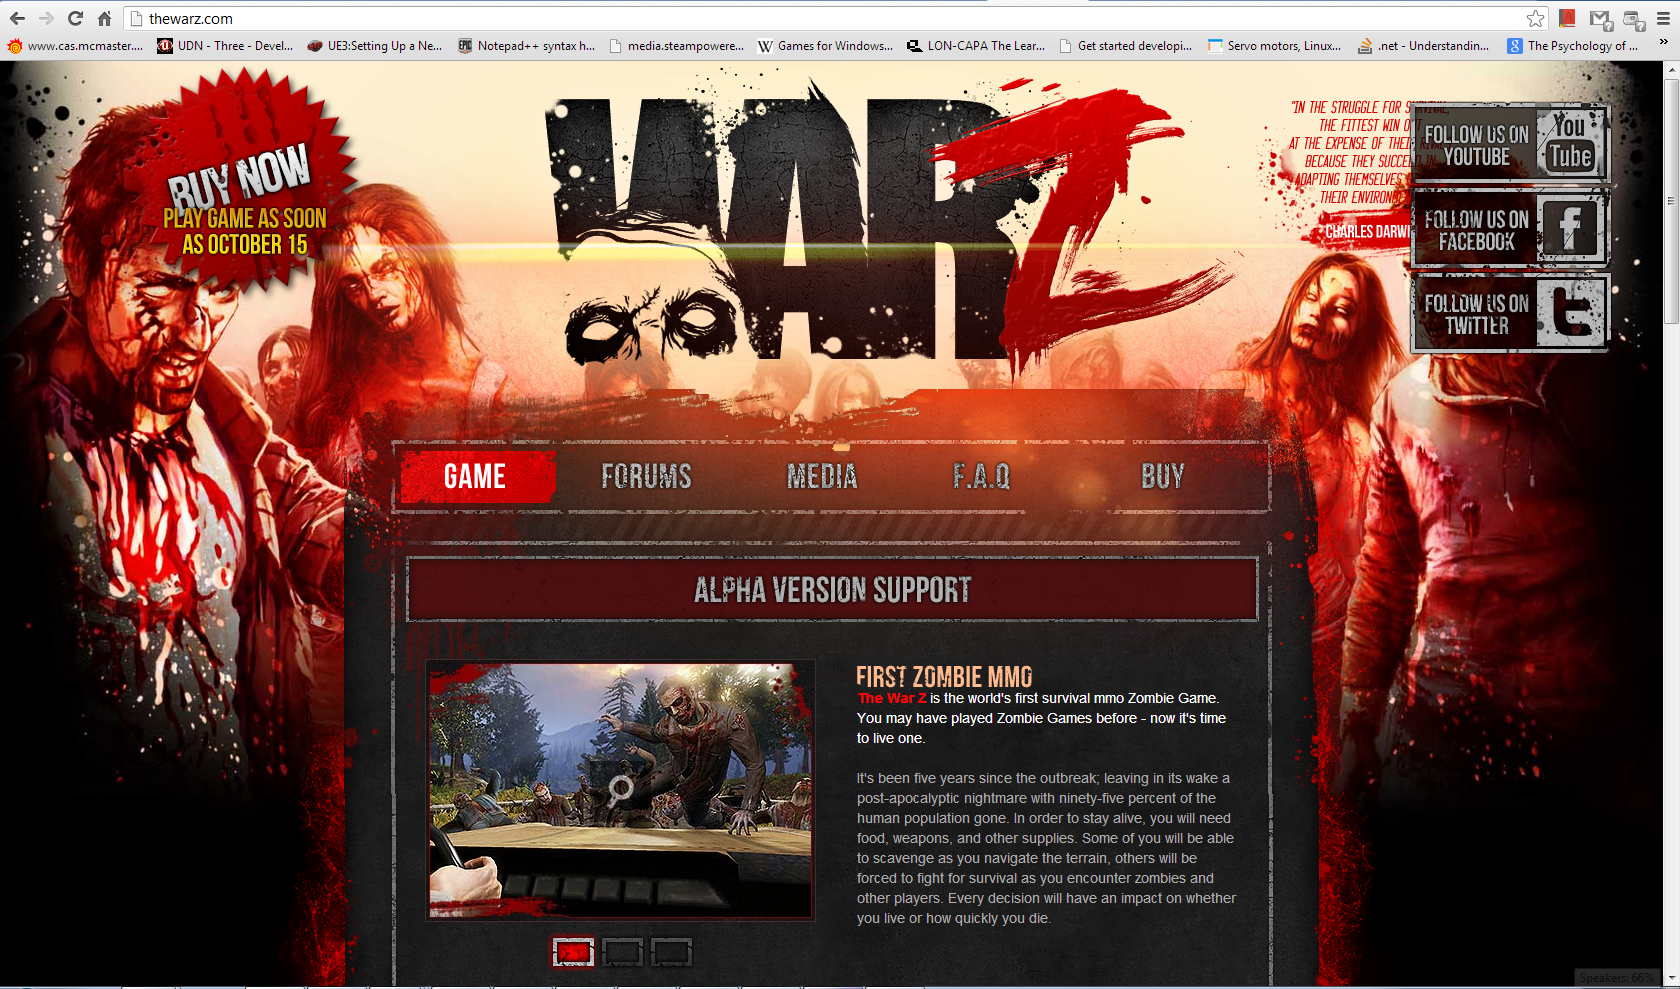
\includegraphics[scale=0.25]{image_1.png}
\end{center}
\caption{Layout of www.thewarz.com}
\label{fig:warzcom}
\end{figure}

\begin{figure}
\begin{center}
\leavevmode
\includegraphics[scale=0.4]{image_2.png}
\end{center}
\caption{Layout of the tutorial module}
\label{fig:warztutmod}
\end{figure}
Since consistency is an important element to UI design, this rule is followed throughout the design of the tutorial module. Graphical images that are going to occur within the game itself are also used often so that future players can easily identify key objects within the game such as landmarks or specific items just through inspection. The font style used on the website is also used in the tutorial module (Arial, 12, white/grey) to keep with consistency. Additionally, the tutorial module will be embedded within a site, viewed using a web browser and the Flash Player add-on, so in the event the site hosting this tutorial module does not look consistent with the game \textit{The War Z}, the Flash itself is self-contained and will continue to have a consistent visual theme regardless of where it is embedded.

\section{Navigation}
The content of the tutorial module is designed in a way that offers simple linear navigation through the different modules (i.e. weapons, equipment, locations, and consumables) however the user can access any part of the tutorial one of two ways. The first way is by selecting a specific module by clicking on the icon associated with the module from section \textit{figure 2.3b} to switch the tutorial to that specific module. The second way to navigate non-linearly is by selecting a step of the current module by clicking on one of the circles from section \textit{figure 2.3a}. These allow the user to skip sections of the specific module and go directly to the step they want to see. By mousing over the buttons one at a time, the user can see what specific section each button leads to by looking at \textit{figure 2.3d}. If the user wants to know which specific module they are currently on, they can look at the centre of the screen, directly below the logo for The War Z at section \textit{figure 2.3c}. Other clear visual indicators of where the user is are also seen in sections \textit{figure 2.3a} and \textit{figure 2.3b}, by looking at which of the icons are currently red as opposed to being faded/greyed out. This presents the user with a clear idea of where they currently are in terms of the context map. Users also have the ability to move linearly as previously stated, this is achieved by using the next and back buttons located at section \textit{figure 2.3f}. When users are on the first step of the first module, there is no back button, just like there is no next button on the last step of the last module.
\begin{figure}
\begin{center}
\leavevmode
\includegraphics[scale=0.35]{image_3.png}
\end{center}
\caption{Tutorial module diagram}
\label{fig:warztutmodlabelled}
\end{figure}

\section{Ease of Use}
In terms of using the actual tutorial module, it is very straight forward and should be easily adopted for use by people who have never played the game \textit{The War Z} before. At the beginning of each specific module, the user will get some insight into the important concepts (introduction) behind that module (i.e. if its about locations, the player will learn about safe buildings to fortify in). When the user is done reading the information on that particular step of the specific module, there is only one \textit{obvious} place to click on, and that's the \textit{next} button. The user will then be presented with a 2-Dimensional menu (as seen in \textit{figure 2.2}) made of icons and a short label of objects/locations relevant to that particular module. This offers the user the ability to easily associate certain visuals with labels for recall when they are actually in the program. The user can then select a specific object or location by pressing on the icons in the 2-Dimensional menu to navigate to a page that explains in greater detail information about the selected object/location. The user can then choose to navigate back to the 2-Dimensional menu by selecting it from \textit{figure 2.3a} or by navigating using the \textit{back} and \textit{next} arrows. If the user is not sure of where to start with a vast amount of information, they can traverse the 2-Dimensional menu of objects/locations linearly by selecting the next arrow, going through each member of the menu one at a time. Each step containing info relevant to a specific object can potentially include an embedded video related to that object (i.e. a 3-D tour of a building). An additional element that can be included for more information feedback is specific object related sound-effects on selection. Since Flash easily supports various media embedding (with their own start, stop, loop, and other controls) the addition of this type of feedback can be easily implemented and offer the user additional information without crowding the limited space provided (i.e. playing what a specific gun sounds like when fired). At the end of each module, the user will be presented with some type of interactive activity to reinforce concepts stated at the beginning of the specific module section. These activities can include quizzes or mini-games. The reason for this way of summarizing a module rather than simply restating the information in a text block is because this online tutorial module is meant to be used for people who are going to \textit{play} a game, and would therefore be more inclined to retain information or even simply enjoy learning through an interactive environment.
\begin{figure}
\begin{center}
\leavevmode
\includegraphics[scale=0.35]{image_4.png}
\end{center}
\caption{Tutorial module 2D-menu member specific information}
\label{fig:warztut2Dmenu}
\end{figure}

\section{Use Case}
In order to gain a greater understanding of how the tutorial module will actually work when being used by a user, this next section will go through a use case of someone learning about the game by completing the \textit{Learning Locations} tutorial module within the Flash project.
\subsection{Learning Locations}
\begin{enumerate}
\item User selects the locations module from the module selection context menu \textit{figure 2.3b}
\item User reads the introduction as seen in \textit{figure 2.3e}
\item User chooses to move to the next step of the \textit{Learning Locations} module by selecting the next button from \textit{figure 2.3f}
\item User sees the 2-Dimensional menu to gather an overview of what is to come in this tutorial module as seen in \textit{figure 2.2}
\item User chooses to see more information about the \textit{church} so they press on the 75 px by 75 px image of the church
\item User reads information about the church and sees a larger image of what the church looks like as seem in \textit{figure 2.4}
\item User skips the remaining step (grocery store) and presses directly on the last step located in \textit{figure 2.3a}
\item User reads the question presented to them and chooses the answer that was most appropriate based on the information read in part (6) by clicking on the answer
\item User sees that their answer was correct as indicated by the large text in green (positive colour reinforcement) in the center bottom of the screen as seen in \textit{figure 2.5}
\item User completes tutorial module \textit{Learning Locations}
\end{enumerate}

\begin{figure}
\begin{center}
\leavevmode
\includegraphics[scale=0.35]{image_5.png}
\end{center}
\caption{Tutorial module quiz}
\label{fig:warztutQuiz}
\end{figure}

\chapter{Appendix}
\section{Flash Actionscript Sample Code}
\subsection{Frame 1}
\begin{verbatim}
stop();
\end{verbatim}
\subsection{Module Selection - Locations Button}
\begin{verbatim}
//The first frame of each scene is specifically labelled as such

on (press) {
	//Scene 3, Frame 1 - Locations Module
	_root.gotoAndStop("3_1");
}
\end{verbatim}
\subsection{Module Step Context Menu - Locations Module - Mouse Over Step 2 Button While on Step 1}
\begin{verbatim}
on (press) {
	_root.gotoAndStop(12); 
	// Frame 12 is Scene 3, Frame 2 
	// Scene 2 * 5 Frames/per scene = 10 
	// 10 Frames + 2 Frames = 12 Frames
}

//Step Name of Button
on (rollOver) {
	_root.dyn_text.text = "LIST OF LOCATIONS";
}

//Current Frame
on (rollOut) {
	_root.dyn_text.text = "INTRODUCTION";
}
\end{verbatim}
\subsection{Quiz Buttons - Grocery Store Answer}
\begin{verbatim}
on (press) {
		var myfont:TextFormat = new TextFormat();
		myfont.bold = true;
		myfont.font = "Arial";
		myfont.size = 20;
		myfont.color = 0x4DFF00;
	if (_root.q_1_title.indexOf("QUESTION 1") != -1)
	{
		_root.q_1_result.setNewTextFormat(myfont);
		_root.q_1_result.text = "CORRECT";
	}
}
\end{verbatim}

\section{Flash Project Workspace}
\begin{figure}[h]
\begin{center}
\leavevmode
\includegraphics[scale=0.25]{timeline.png}
\end{center}
\caption{Flash Time-line}
\label{fig:samplescreenshots2}
\end{figure}

\begin{figure}[h]
\begin{center}
\leavevmode
\includegraphics[scale=0.25]{object_library.png}
\end{center}
\caption{Flash Object Library}
\label{fig:samplescreenshots}
\end{figure}

\end{document}